Un sector circular de radio $r$ y ángulo $\alpha$

\nopagebreak
\begin{align*}
\text{Usando coordenadas polares, el área es:} \\
A &= \int_{0}^{\alpha} \frac{1}{2} r^2 \, d\theta \\
&= \frac{1}{2} r^2 [\theta]_{0}^{\alpha} \\
&= \frac{1}{2} r^2 \alpha
\end{align*}

\[
\boxed{\displaystyle \frac{1}{2} r^2 \alpha}
\]

\begin{center}
    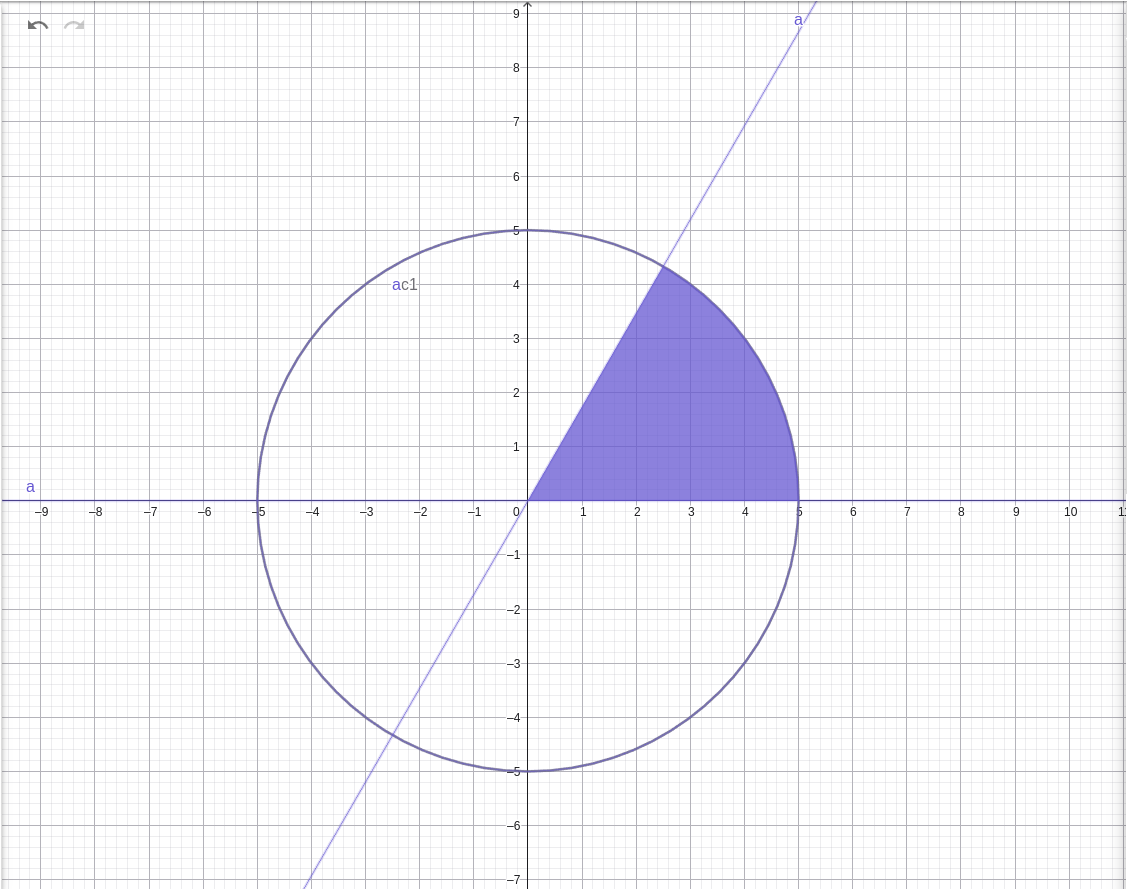
\includegraphics[width=0.5\textwidth]{Graficas/ejer20.png}
\end{center}
